\documentclass[a4paper, oneside]{discothesis}

% use utf8 instead of latin1 when using LaTeX in windows
\usepackage[latin1]{inputenc}
\usepackage[font={small}]{caption}
\usepackage{subfig}


%%%%%%%%%%%%%%%%%%%%%%%%%%%%%%%%%%%%%%%%%%%%%%%%%%%%%%%%%%%%%%%%%%%%%%%%%%%%%%%%%%%%%%%%%%%%%%%%%
% DOCUMENT METADATA

\thesistype{Master Thesis}
\title{Towards Datamarkets with Bitcoin}

\author{Francisc Nicolae Bungiu}
\email{fbungiu@student@ethz.ch}
\institute{Distributed Computing Group \\[2pt]
Computer Engineering and Networks Laboratory \\[2pt]
ETH Z�rich}

% You can put in your own logo here "\includegraphics{...}" or just comment the command
% \logo{}

\supervisors{Christian Decker, Dominic W{\"o}rner, Laura Peer\\[2pt] Prof.\ Dr.\ Roger Wattenhofer}

% You can comment the following two commands if you don't need them
% \keywords{Keywords go here.}
% \categories{ACM categories go here.}

\date{\today}

%%%%%%%%%%%%%%%%%%%%%%%%%%%%%%%%%%%%%%%%%%%%%%%%%%%%%%%%%%%%%%%%%%%%%%%%%%%%%%%%%%%%%%%%%%%%%%%%%

\begin{document}

\frontmatter % do not remove this line
\maketitle

\cleardoublepage

\begin{acknowledgements}
	I thank Lorem ipsum dolor sit amet, consetetur sadipscing elitr, sed diam nonumy eirmod tempor invidunt ut labore et dolore magna aliquyam erat, sed diam voluptua. At vero eos et accusam et justo duo dolores et ea rebum. Stet clita kasd gubergren, no sea takimata sanctus est Lorem ipsum dolor sit amet. Lorem ipsum dolor sit amet, consetetur sadipscing elitr, sed diam nonumy eirmod tempor invidunt ut labore et dolore magna aliquyam erat, sed diam voluptua. At vero eos et accusam et justo duo dolores et ea rebum. Stet clita kasd gubergren, no sea takimata sanctus est Lorem ipsum dolor sit amet.
\end{acknowledgements}


\begin{abstract}

\hspace*{12pt} In recent years, there has been a widespread expansion of data collection and complex methods to analyze such 
collected data. Everyone is constantly generating data by using a large range of computers, smartphones, and gadgets.
In addition, there is an emerging trend towards the Internet of Things technologies that consist
of billions of sensor nodes bridging the gap between the physical and the digital world, and creating massive amounts
of data, but with no incentive to share. 

	In order to provide an incentive for the sensor node owners to share the generated data, these sensor networks
have to initiate data markets that interested customers can subscribe to and pay for the acquired data. Bitcoin provides
an Internet-native payment mechanism and protocols on top of Bitcoin are able to support small payments and avoid 
high cumulated transaction processing costs.

	This thesis proposes a centralized secure scheme that allows data purchasing from any Internet-connected sensor
node using the Bitcoin payments. Based on micropayment channels to aggregate payments and minimize transaction fees, 
and on contracts between the protocol participants to minimize trust, the scheme allows human judgements to be taken
out of the loop and supports complete automation. 
\end{abstract}

\tableofcontents

\listoffigures

\mainmatter % do not remove this line

% Start writing here
\chapter{Introduction}

\hspace*{12pt} The Internet of Things (IoT) is a novel concept that has rapidly expanded in the latest years, refering to the
network formed by any physical object, embedded with sensors and connectivity - such as Radio-Frequency 
Identification (RFID) tags, sensors, smartphones, etc. - that enables such nodes to exchange
data. This technology allows these objects to be sensed and controlled remotely (IoT Survey), having a great
impact on the every-day life of users, and resulting in efficiency and financial benefits.

Sensor nodes with Internet connectivity enable attractive sensing applications in various domains, ranging from
health-care, security and surveillance, environmental monitoring, agriculture automation, energy consumption, transportation, etc.
(Sensing as a Service paper) introduces the concept of Sensing as a Service, in which a number of sensors offer
their generated data as a service to interested entities through a central operator in exchange for a pre-established
price quote. 

Most existing payment protocols for the Sensing as a Service model involve a third-party, which results in higher costs and reduced
efficiency. Another approach is to rely on Bitcoin, a decentralized electronic payment system. 
Bitcoin has at its root the blockchain, a transaction database that is shared by all network 
nodes. However, these solutions fail to address the scalability problem of Bitcoin: 
they rely on atomic operations that are completed directly on the blockchain, thus increasing its size and moving Bitcoin
towards centralization, since only a few nodes will be able to process a block. 

IoT has a huge economic potential and areas of application include: road surveillance - interested in road condition data generated by cars (Nericell, VTrack), 
weather forecast - in data sensed by private weather stations, transportation - paying per distance or number of bus stops, 
paying for Internet by used traffic, etc. 
In this manner, IoT entities can act as active participants in a self-created data market. However, it is still lacking
an efficient payment method and is limited by high transaction costs.

In this context, the project proposes a centralized, low-trust and secure scheme that allows and incentivizes sensor nodes
to share sensed data and get paid in exchange in bitcoins. The presented solution utilizes micropayment channels
to solve Bitcoin's scalability problem by bundling several small payments for each set of acquired data and only
publishing the final, aggregated transaction to the network. In order to confer a low-trust relation between the system 
entities, the protocol relies on contracts that pass the payment obligation down from the buyer to the central coordinator,
and then to the sensor node. In addition to the theoretical model, a proof-of-concept is built based on the Android built-in
sensors.

\section{Background}

In the following sub-sections, the background on the used concepts and sub-protocols is presented.

\subsection{Bitcoin}

\hspace*{12pt} Since its invention in 2008 [Satoshi paper], Bitcoin has grown into a global electronic payment system.
It uses peer-to-peer technology to transfer funds, with no need for a central authority such as a financial institution
and low transaction fees, making it an attractive alternative to traditional payment methods.
A proof-of-work system and cryptographic protocols are the building blocks of the protocol, with peers participating
in the network being responsible for processing transactions and issuing of bitcoins. 

\vspace*{5pt}
\begin{figure}[!ht]
  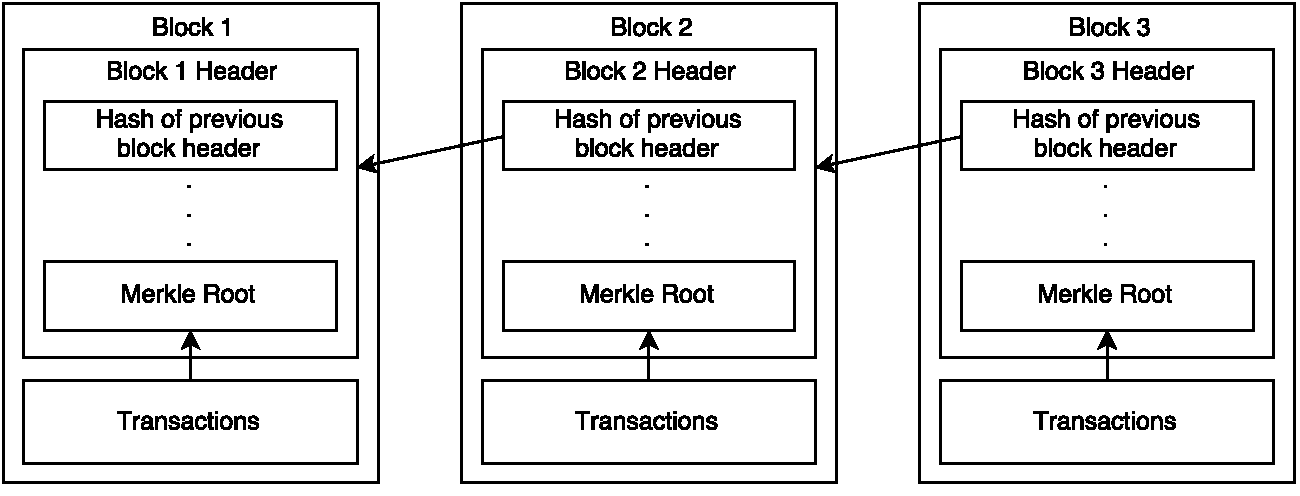
\includegraphics[width=\textwidth]{figures/Blockchain}
  \caption{A simplified representation of the Bitcoin blockchain.}
\end{figure}

Bitcoin relies on public key cryptography to authenticate transactions. Each peer in the network has one or more 
public and private key pairs that are stored in a file called a wallet. In order to support and authenticate transactions, 
an address is derived from the public key and is disclosed together with it to the participants.
In this cash system, transactions consist of one or more inputs (references to previous transaction outputs)
assigning the value of all inputs to one or more outputs. An output consists of a tuple of a specified
bitcoin amount, and an output script, called pubscript. This special script describes conditions
that need to be satisfied in order for the amount to be claimed by an entity. In most cases,
the script only requires a signature matching the address, which proves the possession of the 
corresponding private key. The difference between the total input amount and the total
output amount in a transaction represents the transaction fee.
A peer holding a private key can sign a transaction spending some of its wallet's amount to some other address, and 
any other peer that sees this transaction can verify the signature using the peer's public key. In order to claim an
output, the payee must prove that it possesses the private key corresponding to the public key included as the destination
of the transaction. Thus, the available funds are represented by the amount of all unspent transaction outputs the peer possesses a private key for.

In order to be validated and accepted by the peers, 
a transaction needs to be broadcast to the network. Special network nodes, called miners, will then timestamp it by applying a hash function into
a continuously growing chain of hash-based proof-of-work. This forms a record, called the blockchain, containing
all transactions in Bitcoin ever made, that cannot be changed without redoing the entire proof-of-work.
The public ledger is distributed to all network peers and is crucial for protection against 
double spending and modification of older transactions. The proof-of-work performed in Bitcoin is based on HashCash POW [cite],
which means new blocks (containing one or more transactions) are only accepted into the ledger 
if the hash of the block header contains a specified number
of zeros as a prefix (adapted dynamically to produce bitcoins at a constant rate). 
The header of each block contains, among other data, a 4-byte nonce, that miners permute until 
the hash fulfills the criteria. Once it does, the new block is broadcast to the network and verified by the other peers
before being added to the blockchain. This PoW takes advantage of the random nature of cryptographic hashes, making it
impossible to modify the data to obtain predictable hashes. The computation, called mining, is incentivized through fees
that are earned by the nodes performing it.

\subsection {Micropayment channels}

\hspace*{12pt} Unlike traditional payment methods, Bitcoin transactions are very cheap in terms
of fees, but still have a considerable cost given the mining and storing they require. The context
of Internet of Things requires a high volume of small-value payments, thus the overall fees
might reach and surpass the value of the actual transactions. In addition to this, broadcasting
several transactions to the Bitcoin network in a very short time window will trigger network anti-flooding
algorithms, which will result in either the transactions being delayed or, even worse, not relayed. 
Last, the payee of such small transactions will end up with a wallet full of ``dust'', and spending
such money is expensive fee-wise.

To address these issues, the construct of payment channels was introduced in Bitcoin. After an initial
setup process between the two participants, the payer can start sending tiny payments to the other party
off the blockchain at high speed, without paying high transaction fees, in a trust-free manner.

\vspace*{5pt}
\begin{figure}[!ht]
  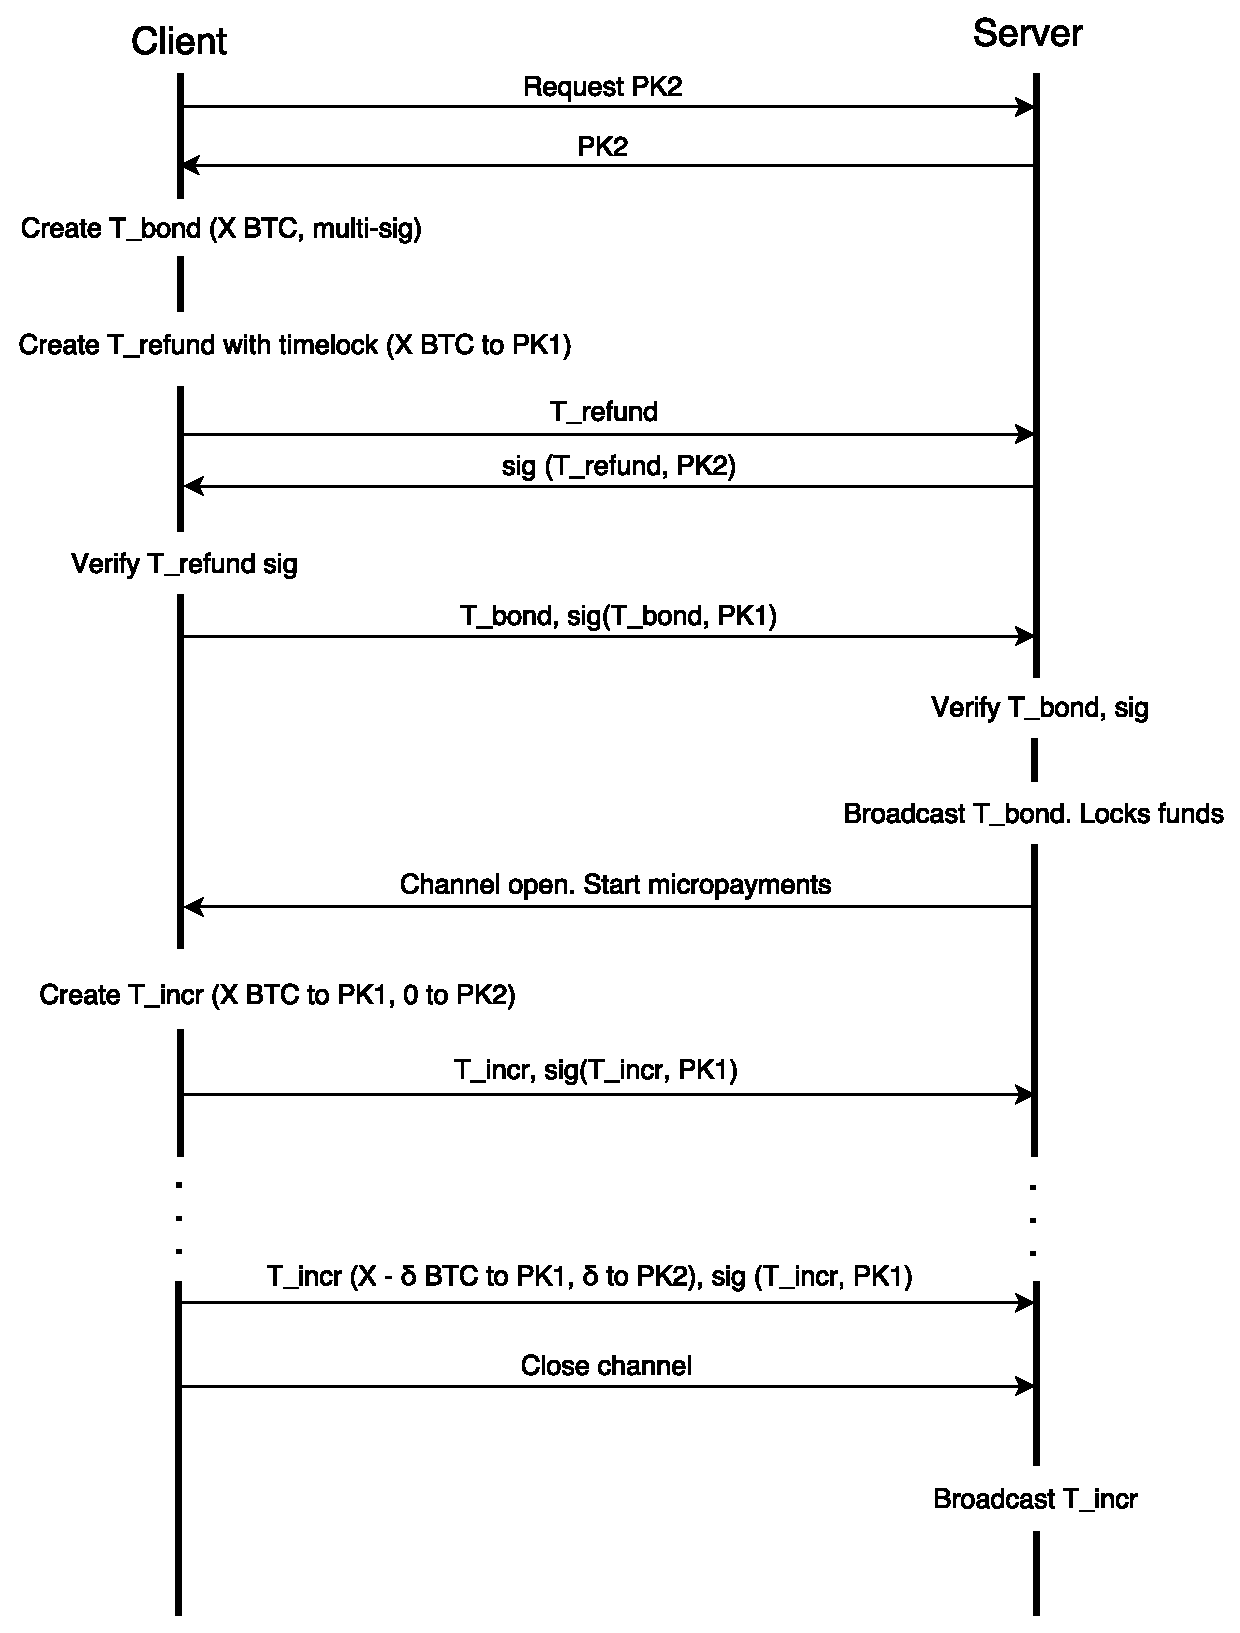
\includegraphics[width=\textwidth]{figures/MicropaymentSeq}
  \caption{Micropayment channel protocol: setting up the shared account (bond transaction), creating the refund 
  transaction, and updating the incremental payment transaction.}
\end{figure}

Consider a buyer that is interested in data generated by sensor nodes in a IoT network.
In exchange for the obtained data, it will pay the data provider in bitcoins. Since none of the
participants know each other, a zero-trust solution is necessary to reassure both the buyer that it will
not lose its bitcoins in case the sensor node does not provide the data, and that the sensor node will
not provide the promised service without getting remunerated. The construct works in two stages.
First, the buyer creates a multi-signature transaction, a shared account requiring signatures
of both participants to spend from it, that pre-allocates a certain amount of 
bitcoins for use in the channel. If the buyer signs and sends this bond transaction to the sensor node,
the node could simply broadcast it and keep the money hostage, thus the buyer keeps the transaction
private for now and creates another one, called a refund transaction, and sends it to the other
peer to sign it. This transaction refunds the
entire value to the buyer, but it time locked using the nLockTime feature of Bitcoin,
ensuring it will not become valid until some time in the future (channel lifetime). 
If the sensor node vanishes at any point, the buyer can then use the refund transaction 
to get all the money back at channel expiration time.

Once the refund has been signed by the sensor node, the buyer can safely send the signed bond transaction.
After verifying the signature, the server signs it as well and broadcasts it to the network, locking
in the money and opening the channel between the two parties. 

At this point, the work-and-pay cycles can begin. Initially, the buyer creates a new transaction
spending from the shared account and adds two outputs: one to its own address with the full amount, 
and one to the address of the payee. After signing it, the buyer sends it to the peer. 
When new data is requested from the data provider, the transaction is updated by the buyer, with increasing
value to the sensor node and decreasing value allocated to its own address. In each update cycle, the
transaction is signed and handed over to the other party. 
When the time comes and the buyer wishes
to close the channel, it notifies the sensor node, which in turn signs the transaction with the 
highest value alloted to it and broadcasts it to the network. This step closes the channel, unlocking
the buyer's remaining money and making the sensor's money available for spending. The buyer could be
tempted to broadcast an older transaction that gives less money to the sensor node than it deserved
for the provided data, but it is missing the sensor's signature. Thus, the construct of micropayment
channels prevents misbehavior from both parties.

\subsection{Hashed Time-Lock Contracts (HTLCs)}

\hspace*{12pt} Since the project proposes a three-component system in which payments need to be forwarded
from the buyer all the way to the data sensor nodes, a blockchain enforced contract needs to be set in place
in order to prevent the intermediaries from delaying or keeping these funds for themselves.

To create an HTLC, a special HTLC setup transaction is set up that can only be claimed 
by the final recipient {\it B}  of the payment using a previously created secret.
First, the payee {\it A} has to generate a secret {\it R} and hash it to obtain {\it H}. 
Then {\it H} and the recipient's Bitcoin address are directly transferred to the payer. 
At this step, all nodes on the  payment path between the sender and the recipient
need to create HTLC setup transactions connected to the output of a shared account 
using the provided hash H. The output of the HTLC setup contains a pubScript as shown in
\ref{fig:htlcpubscript}, which requires
a signature from both participants (first branch), or the next hop provides {R'} such that
it hashes to {\it H}.
Once all setup transactions are in place, the recipient {\it B}
can release {\it R} to claim the funds from the previous node. The secret is then revealed
step by step by all nodes on path all the way back to {\it A}, which completes the transfer.

\vspace*{5pt}
\begin{figure}[tbp]
  \centering
    \subfloat[HTLC pubScript.]{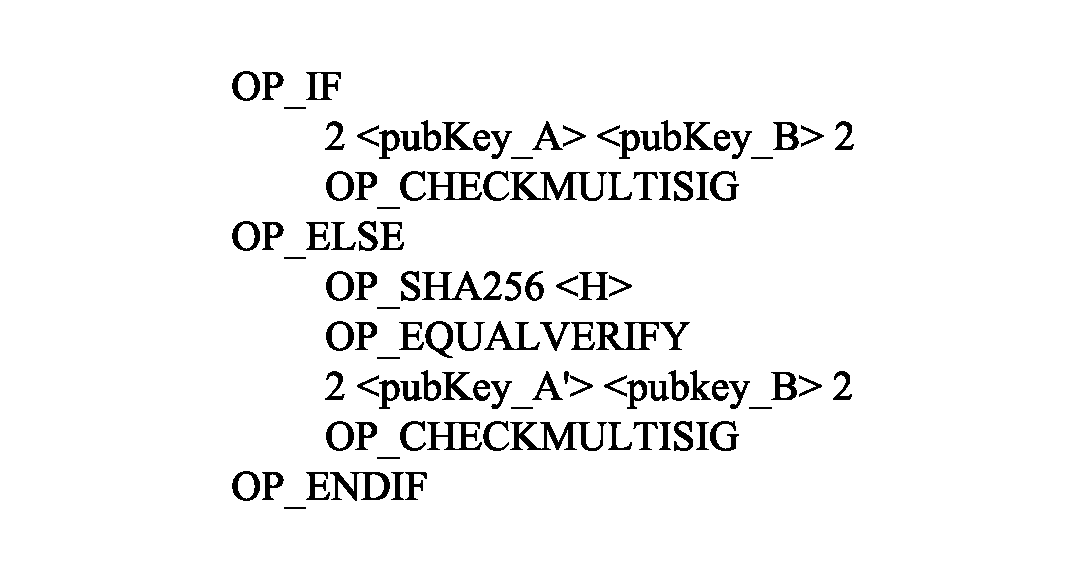
\includegraphics[width=0.5\textwidth]{figures/HTLCPubScript}
    \label{fig:htlcpubscript}}
    \subfloat[HTLC Transaction structure.]{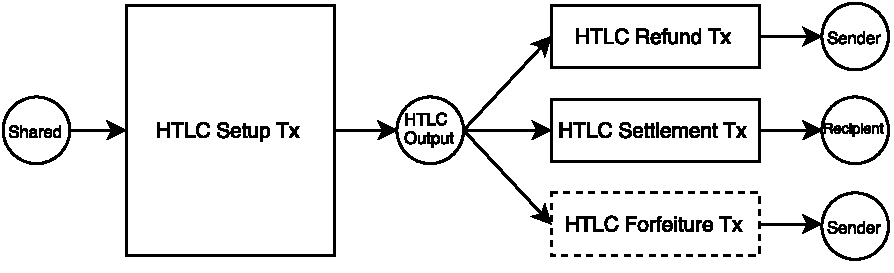
\includegraphics[width=0.5\textwidth]{figures/HTLCTxs}
    \label{fig:htlctxstructure}}
\end{figure}

To prevent the intermediaries from delaying the funds, stealing or keeping them hostage, 
HTLC refund, settlement and sometimes forfeiture transactions are created, all three types
claiming the HTLC output. 
The {\it HTLC refund} transaction is similar to the refund that is created in the micropayment
channel setup protocol, but has a higher time lock to give the sender enough time
to react, should the receiver not cooperate.
The {\it HTLC settlement} transaction guarantees the receiver it can pull the funds if it 
is in the posession of the secret. It is important for the sender to use different signing keys
{\it A} and {\it A'} for the two branches of the HTLC output. Otherwise, the receiver 
could simply reuse the signature of the settlement transaction in the if-branch and claim
the funds without ever revealing the secret, since the signature is valid for the entire pubScript.
Lastly, the {\it forfeiture transaction} addresses the case in which the sender and the
receiver agreed to void the HTLC and remove the output. If the receiver comes in possession
of the secret at a later stage, it still has the signed settlement transaction that it 
could simply broadcast and steal the bitcoins. Because of this, every time the receiver
backs off from the HTLC, it creates and hands over a forfeiture transaction that transfers the bitcoins
back to the sender. Should the receiver broadcast an older setup transaction,
the sender can simply use the forfeiture to get the money back.

%Notes: 
% reputation systems
% bitcoin soft-fork from Lightning to secure the protocol
% Android device can encrypt data with the buyer's pubkey  + secret : onion, or ECDSA

\section{Related work}

\hspace*{12pt} Following the expansion trend of the Internet of Things technologies, there has been an increasing interest in 
creating secure payment protocols that allow customers to acquire sensor data efficiently. 

(IoT based on the Protocol of Bitcoin paper) introduces a new low-trust E-business architecture that is tailored 
for IoT. This architecture is based on Bitcoin, eliminating the need for a 
third-party in the process. In order to make a payment and receive the data in exchange, the buyer and the data provider 
make an offer-proposal exchange, then build a transaction that spends the required amount and publish it to the network. 
A similar approach is proposed in (When Money learns to fly), where the encrypted data is directly included in the 
blockchain after a payment is made, which only the buyer in possession of the corresponding private key can decrypt.
In both approaches, all transactions, no matter how small, need to be published to the network, which results in high 
cumulated fees and time-wise inefficiency, thus being directly affected by the scalability problem of Bitcoin (cite).

Work has also been done on micropayment protocols that reduce fee costs.
Amazon Flexible Payment Service uses a central provider that aggregates 
clients' micropayments into macropayments that are flushed to the seller at specific times. This solution
does not provide anonymity, since the central provider can keep track of all payments, and moreover,
was discontinued on June 1, 2015.
Other protocols (Micropayments Revisited) involve a probabilistic approach. Using a selection rate {\it s}, it
discards all unselected micropayments and selects one with probability {\it s} that can be deposited for an amount
{\it 1/s} times bigger than the original amount. This should ensure everyone gets, on average, the expected amount. 
However, this solution lacks anonymity, requires PKI certificates and comes closer to a bet than an actual transaction.

The Architecture of Coupon-Based, Semi-off-Line Anonymous Micropayment System for Internet of Things - 
proposes an anonymous, semi-offline micropayment system for transactions in IoT. In this approach, an electronic
coin is obtained by iteratively applying a hash function to some initial seed, thus allowing the user to spend it
in fractions, by presenting a set of hash chain nodes to the vendor. 
The protocol is designed to meet the needs of IoT transactions, however, it has limited potential to be implemented because it does 
not rely on an existing financial institution. 
Another coupon-based system has been proposed by Rivest in [PayWord and MicroMint] and was improved by Payeras-Capella 
(An efficient anonymous...) to integrate anonymity and prevent users from exceeding their account limit. The drawback of the
latter is that the financial institution needs to be contacted directly before each payment, and any unspent value is lost
in favor of the financial institution. Wilusz (Requirements and general..) solves these issues by requiring a single 
contact with the financial institution at coin issue time and allowing the user to use unspent fractions in future transactions.
However, a clearing house is necessary to lock in the coin by the vendor, which increases transactions costs, 
and poses the risk of locking the coin indefinitely.

There have been some previous projects that utilize micropayment channels to pay in bitcoins in exchange for services. 
[Paying for Internet one byte] is a proof-of-concept allowing an access point to provide Internet access to 
untrusted users for bitcoins through a micropayment channel in a convenient manner. This way owners are incentivized
to open up their access points and users receive Internet services in return. Though the idea of using micropayment
channels for several small-valued transactions does address the scalability problem of Bitcoin, establishing micropayment
channels between all pairs of buyers and service providers is rather inefficient in the context of this project.

It is worth mentioning that there have been several proposals and ideas that can be exploited to support
trustless, instant, off-the-chain Bitcoin payments
on bitcointalk.org by Mike Hearn, Alex Akselrod, hashcoin, Meni Rosenfeld, cjp, Tier Nolan etc.

On the Contracts page of Bitcoin, Mike Hearn (https://en.bitcoin.it/wiki/Contract\#Example\_2:\_Escrow\_and\_dispute\_mediation) describes an idea
on how to trade with somebody with no trust involved, based on multi-signature transactions. The funds get locked in a shared account
controlled by at least two of the three participating parties: the client, merchant and mediator. If the transaction is successful
or a refund is agreed upon, the client and the merchant can move funds. If the trade fails, the client and the mediator can agree,
and a charge-back occurs. Finally, if the goods are delivered but the client does not want to fulfill its part of the agreement,
the mediator and the merchant agree and the merchant gets the client's money. Mike also proposed the idea of trading across
multiple currencies without a third party, and Tier Nolan formalized it in a protocol that allows the exchange atomically, using
time locks and hash commits.

cjp presented a draft that combines Bitcoin and Ripple to create a high-speed, scalable, anonymous, decentralized, low-trust
payment network. In this Bitcoin-specialized variation of the Ripple system, neighboring pairs
have a shared account that is partly allocated to one of them, and the rest to the other, as agreed
between the two, which lowers the needed trust. Using sequence numbers to update this transaction
as payments in the network are made and lock times to prevent blocking the money indefinitely. 

Meni Rosenfeld proposed
a simple way of reusing existing micropayment channels instead of establishing new ones if a path between
the payer and the payee already exists. The intermediaries would then only be trusted with the amount of a single payment
from a single buyer. 

Alex Akselrod - Extensible Scalable Coopetitive High Availability Trade Optimization Network - built a proof-of-concept
for chained micropayment channels with two-phase commits. The original micropayment channel payment scheme is modified
to allow sending funds through intermediaries. Suppose Alice, Carol, and Bob have previously set-up micropayment channels
pairwise, in the given order. If Alice wants to send bitcoins to Bob through Carol, Bob first creates
a random secret R, hashes it and sends the commit hash to Alice out-of-band. Then Alice can update the values on the
channel with Carol using the commit hash, and Carol can do the same on the channel with Bob. In order to claim the money,
Bob has to reveal the secret to Carol, and Carol can then reveal the secret to Alice up the path to receive her funds.
Thus, this proposal enables friend-to-friend, instant, off-blockchain, trustless payments of arbitrary size using Bitcoin
micropayment channels.

Peter Todd's proposal in Hub-and-Spoke Payments provides the an efficient way for establishing micropayment
channels between peers with a central hub. This central entity plays the role of a router, basically fowarding
payments from the payer to the payee. Suppose Alice and Bob have previously established micropayment channels with
the hub. If Alice wishes to send bitcoins to Bob, she should normally establish a new micropayment channel with him.
However, both of them have channels opened with the hub, so Alice can send the funds to the hub, and the hub can then
forward the payment to Bob. Using Hub-and-Spoke payments, payments between buyers and service providers with a central
coordinator can be made efficiently, saving costs in terms of fees. However, the forwarding process should be enforced and secured,
part that is noted in the proposal, but without specifying an actual way to do so. 

The Lightning Paper presents a promising solution to Bitcoin's scalability problem and provides a way to
securely forward payments on a path of peers through blockchain enforced contracts. 
It solves the issue by using timelocks on a network of micropayment channels combined with Hashed Timelock Contracts (HTLC) 
- recipient generates random data R, hashes it to produce H and sends H to the sender of funds, together with its bitcoin address. 
Sender routes its payment to the receiver and when an updated transaction is received, the recipient may elect to redeem the 
transaction by disclosing the random data R (which pulls the funds from the sender).
With the introduction of a new sighash
type which solves malleability, the proposed protocol allows offchain transactions between untrusted parties with fully enforceable
contracts, making Bitcoin scale to billions of users.

For the sake of completeness of this literature review, we mention the TilePay project, which promises a decentralized
payment system based Bitcoin for real-time access to IoT sensors, based on micropayments. In a partnership
with Cryptotronix, TilePay wants to enable cryptocurrency payments to IoT devices. However, since the announcement
in December 2014, no work or detailed information on how they would achieve that has been published.

\chapter{Design}

\section{Requirements}

\hspace*{12pt} For the presented use case, a scheme that enables sensor nodes in an Internet-of-Things network to shared sensed data and 
get paid in exchange must meet the following requirements:
\begin{itemize}
 \item Provide an entity that the node can register sensor type availability to.
 \item Provide an entity that buyers can query for available data and that can provide sensor node contact
 information
 \item Scalability: avoid broadcasting all micro-transactions to the blockchain
 \item Efficiency (and speed): fast communication between components, payments and data should be confirmed and received instantly
 \item Secure: end-to-end security of the payments
 \item Anonymous: linking of buyers and sellers and identification across sessions should not be possible.
\end{itemize}

\subsection{Achieving Scalability and Efficiency}

\hspace*{12pt} In order to achieve scalability and efficiency, there are two important factors that need to be taken
into account: the inherent scalability issue of Bitcoin and the number of peer pairs that need
to interact to successfully get payments from buyers to the sensors.

Since sensor nodes are exchanging small sets of sensed data in exchange for bitcoins, individual payments
made by the buyer tend to be of very small amounts. Therefore, creating new transactions for each
such payment would have a very high overhead in terms of fees, which reduces the incentive for
both the buyers and the sensor nodes to participate in the protocol. A high volume of transactions
would also delay the transactions being confirmed on the Bitcoin network. To address these
issues, the proposed system will rely on the previously introduced micropayment channels. 
This mechanism will allow, after a preliminary setup between the parts that wish to transact,
to instantly send small amounts of bitcoins off the blockchain, bundling and publishing them to the
network only at the end of a specified time window. Thus, both scalability of Bitcoin and efficiency
of payments are achieved.

One issue that comes with using micropayment channels in the proposed context 
is that its set-up phase takes a considerable time (approximately 10 minutes, until the bond transaction
is confirmed by the network). Thus, setting up a channel between all buyers and nodes becomes 
very inefficient time-wise and causes a lot of overhead on the network since all connections need
to be maintained for the lifetime of the channel.
On the other hand, if the buyers and the sensors
have previously established a channel with a central entity as in the hub-and-spoke model (cite), 
each will have a single set-up to wait for and a single channel 
connection to maintain. To better illustrate the performance improvement, suppose the system runs
{\it X = 100} buyers and {\it Y = 100} data providers. By using the initial idea, {\it X*Y = 10.000} 
channels  need to be established and maintained. With the hub-and-spoke model, however, 
{\it X + Y = 200} channels will suffice (factor of {\it 50}).

Last, adding a single central entity may affect the scalability of the system when the number of 
data providers and buyers increases, becoming a performance bottleneck. 
However, the concept of a central hub should be rather
treated as a central cloud, which can contain several machines maintaining the connections,
channels, available sensor data, and load balancers that distributed the work across the available
machines.

\subsection{Achieving Security}

Talk about micropayment channels + HTLCs. Sequence diagram for full protocol.

\subsection{Achieving Anonymity}

By design, the role of the central hub is to connect data buyers and sellers, and given that
the lifetime of the established micropayment channels are rather long, the hub can easily analyze
the data a buyer is interested in, build a profile and ultimately, identifying it. To address
the privacy issue, buyers could make use of a distributed 'onion' network, such as Tor,
open several, shorter-lived sessions, over several vantage points, 
and spread payments and data exchanges on these session when buying different sets of data. 
An additional precaution is to never reuse addresses across sessions. 
This way, profiling becomes more difficult,
and the hub can not link anymore buyers and data they have purchased through the system.

\section{System Overview}

The design of the payment system achieving the requirements above comprises three major components:
one component consists of several sensor data providers (IoT sensor nodes, Android phones
running specialized app, etc.), one central hub that plays an essential role in sensor node discovery
and payment and data relaying, and a third component, consisting of data buyers. The communication
between the buyers and the hub, and between the hub and the sensor nodes is done through TCP links.

\begin{figure}[!ht]
  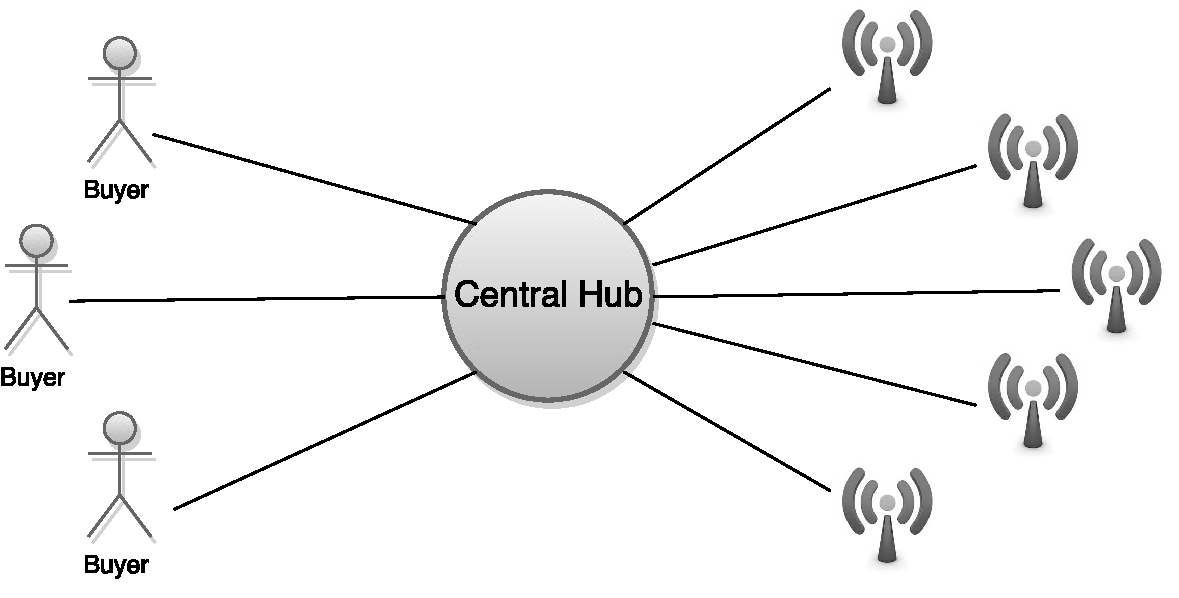
\includegraphics[width=\textwidth]{figures/SystemOverview}
  \caption{System overview: buyers, central hub, and sensor nodes.}
\end{figure}

\section{System components}

\subsection{Buyers}

\subsection{Central Hub}

\subsection{Sensor nodes}



\chapter{Implementation}

\chapter{Evaluation}

\chapter{Conclusion}

\chapter{References}

% This displays the bibliography for all cited external documents. All references have to be defined in the file references.bib and can then be cited from within this document.
\bibliographystyle{splncs}
\bibliography{references}

% This creates an appendix chapter, comment if not needed.
\appendix
\chapter{Appendix Chapter}

\end{document}